% ============================================================
%  Chapter 4: Experiments
% ============================================================

\chapter{Experimental Setup}
\label{ch:experiments}

This chapter describes the experimental protocol used to evaluate
\modnet{}. We begin with the six benchmark tasks, then describe the
data encoding, the evaluation procedure, the hyperparameter choices,
and finally the reproducibility of the experiments.

% ------------------------------------------------------------
\section{Benchmark Tasks}
\label{sec:tasks}
% ------------------------------------------------------------

We evaluate \modnet{} on six tasks that span two broad classes:
Boolean function learning and continuous regression. The tasks were
chosen to cover a spectrum of difficulty, from problems that are
trivially solvable by a single linear unit (XOR) to problems that
require multi-stage nonlinear computation (6-bit parity). Table~\ref{tab:tasks}
summarizes the tasks; Figure~\ref{fig:tasks} illustrates the two
regression tasks.

\subsection{Boolean Function Learning}

Boolean function learning is a natural testbed for \modnet{} because
the fitness function is exact (there is no measurement noise) and the
correctness of the result is unambiguous. We use three Boolean tasks.

\begin{itemize}
  \item \textbf{XOR (2-bit).} The exclusive-or of two bits,
    $\text{XOR}(a, b) = a \oplus b$. XOR is the canonical example of
    a non-linearly-separable Boolean function: no single linear
    threshold unit can compute it \citep{minsky1969perceptrons}.

  \item \textbf{Parity (4-bit).} The parity of four bits,
    $\text{Parity}_4(\mathbf{x}) = \bigoplus_{i=1}^{4} x_i$. Parity
    is the XOR of $n$ bits and is the simplest Boolean function that
    is provably hard for bounded-depth threshold circuits: any depth-$d$
    circuit that computes parity requires $\Omega(n^{1+\varepsilon_d})$
    wires \citep{impagliazzo1997size}. For $n = 4$, the function has
    $2^4 = 16$ input--output pairs, eight with output $0$ and eight
    with output $1$.

  \item \textbf{Parity (6-bit).} The parity of six bits,
    $\text{Parity}_6(\mathbf{x}) = \bigoplus_{i=1}^{6} x_i$. This is
    a harder version of the previous task: it has $2^6 = 64$
    input--output pairs, and the number of pairs grows exponentially
    with $n$.
\end{itemize}

For all three Boolean tasks, the target values are encoded as a
single bit, and the fitness is the mean squared error between the
predicted bit and the target bit (Section~\ref{sec:fitness}).

\subsection{Continuous Regression}

Continuous regression tasks test whether \modnet{} can produce smooth,
graded outputs rather than binary decisions. We use three regression
tasks.

\begin{itemize}
  \item \textbf{sin(2\texorpdfstring{$\pi$}{pi}x).} A single sinusoid
    over the unit interval, normalized to $[0, 1]$:
    \[
      y(x) = 0.5 \cdot \sin(2\pi x) + 0.5.
    \]
    We sample $N = 32$ points uniformly at random on $[0, 1]$. This
    task has a single input dimension and a single output dimension,
    but the output is a periodic function that requires fine-grained
    reproduction.

  \item \textbf{sin(4\texorpdfstring{$\pi$}{pi}x).} A sinusoid of
    twice the frequency, again normalized to $[0, 1]$:
    \[
      y(x) = 0.5 \cdot \sin(4\pi x) + 0.5.
    \]
    The higher frequency makes this task harder: the network must
    reproduce a function that oscillates twice as fast over the same
    interval.

  \item \textbf{Circle ($x^2 + y^2$).} A two-dimensional quadratic
    surface:
    \[
      y(x_1, x_2) = 0.5 + 0.25 \cdot (x_1^2 + x_2^2).
    \]
    We sample a $5 \times 5$ grid over $[0, 1]^2$, giving $N = 25$
    points. This task has two input dimensions and a single output
    dimension, and the target function has a nontrivial curvature in
    both input coordinates.
\end{itemize}

For all three regression tasks, the target values are quantized to
$2^{8} = 256$ levels and encoded as $8$-bit binary vectors. The
fitness is the mean squared error between the decoded output and the
target value.

\begin{table}[h]
  \centering
  \small
  \caption{Summary of benchmark tasks.}
  \label{tab:tasks}
  \begin{tabular}{llrrrl}
    \toprule
    \textbf{Task} & \textbf{Type} & $n_{\text{in}}$ & $n_{\text{out}}$
      & $N$ & \textbf{Description} \\
    \midrule
    XOR2      & Boolean    & 2 & 1 &  4 & $a \oplus b$ \\
    Parity4   & Boolean    & 4 & 1 & 16 & $\bigoplus_{i=1}^4 x_i$ \\
    Parity6   & Boolean    & 6 & 1 & 64 & $\bigoplus_{i=1}^6 x_i$ \\
    sin2pi    & Regression & 4 & 8 & 32 & $0.5 + 0.5\sin(2\pi x)$ \\
    sin4pi    & Regression & 4 & 8 & 32 & $0.5 + 0.5\sin(4\pi x)$ \\
    Circle    & Regression & 8 & 8 & 25 & $0.5 + 0.25(x_1^2 + x_2^2)$ \\
    \bottomrule
  \end{tabular}
\end{table}

\begin{figure}[h]
  \centering
  \begin{subfigure}[b]{0.48\textwidth}
    \centering
    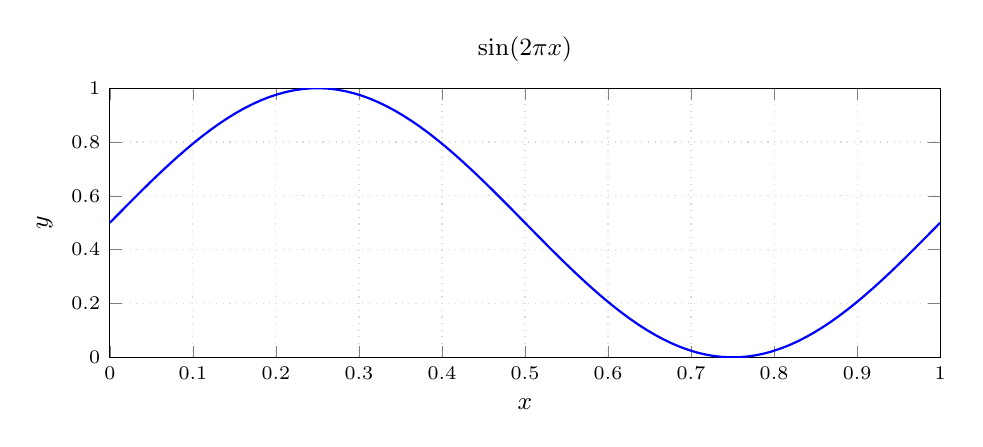
\begin{tikzpicture}
      \begin{axis}[
        width=\textwidth, height=5cm,
        xlabel={$x$}, ylabel={$y$},
        xmin=0, xmax=1, ymin=0, ymax=1,
        grid=major, grid style={dotted,gray!30},
        title={sin($2\pi x$)},
        title style={font=\small},
        tick label style={font=\scriptsize},
        label style={font=\small},
      ]
        \addplot[blue, thick, samples=100, domain=0:1]
          {0.5 + 0.5*sin(deg(2*pi*x))};
      \end{axis}
    \end{tikzpicture}
    \caption{sin(2$\pi$ x), N=32 samples.}
    \label{fig:task-sin2pi}
  \end{subfigure}
  \hfill
  \begin{subfigure}[b]{0.48\textwidth}
    \centering
    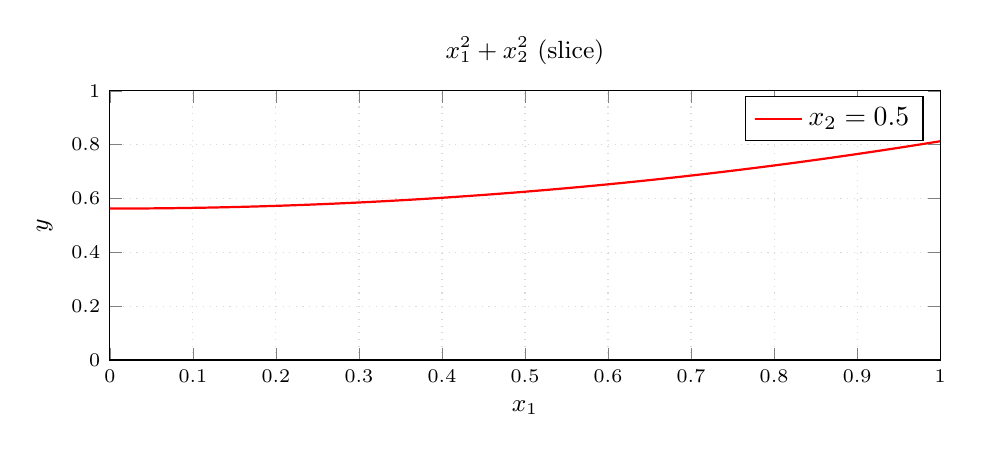
\begin{tikzpicture}
      \begin{axis}[
        width=\textwidth, height=5cm,
        xlabel={$x_1$}, ylabel={$y$},
        xmin=0, xmax=1, ymin=0, ymax=1,
        grid=major, grid style={dotted,gray!30},
        title={$x_1^2 + x_2^2$ (slice)},
        title style={font=\small},
        tick label style={font=\scriptsize},
        label style={font=\small},
      ]
        \addplot[red, thick, samples=100, domain=0:1]
          {0.5 + 0.25*(x*x + 0.25)};
        \addlegendentry{$x_2 = 0.5$}
      \end{axis}
    \end{tikzpicture}
    \caption{$x_1^2 + x_2^2$ at fixed $x_2 = 0.5$.}
    \label{fig:task-circle}
  \end{subfigure}
  \caption{Illustration of the two regression task families. Left:
    the sinusoid used in \texttt{sin2pi} and \texttt{sin4pi}. Right:
    a slice of the quadratic surface used in \texttt{circle}.}
  \label{fig:tasks}
\end{figure}

% ------------------------------------------------------------
\section{Data Encoding}
\label{sec:encoding}
% ------------------------------------------------------------

Inputs and outputs of \modnet{} are binary vectors. Continuous values
are quantized to a fixed number of bits, as follows.

\subsection{Boolean Inputs}

For Boolean tasks, each input bit is passed directly to the network
as a $0$ or $1$ value. No encoding is required.

\subsection{Continuous Inputs}

For regression tasks, each continuous input variable $x \in [0, 1]$
is quantized to $b$ bits as follows. Let $v = \lfloor x \cdot (2^b - 1) \rceil$
be the rounded integer in $[0, 2^b - 1]$. The bit vector is then

\begin{equation}
  \text{encode}(x, b) = \left( \lfloor v / 2^0 \rfloor \bmod 2, \,
                            \lfloor v / 2^1 \rfloor \bmod 2, \,
                            \ldots, \,
                            \lfloor v / 2^{b-1} \rfloor \bmod 2 \right).
  \label{eq:encode}
\end{equation}

We use $b = 4$ bits for inputs, giving $2^4 = 16$ distinct input levels
per variable. This is a coarse quantization, deliberately chosen to
keep the input space small enough for exhaustive evaluation: with $n$
input variables, the total number of distinct inputs is $2^{4n}$.

\subsection{Outputs}

For Boolean tasks, the output is a single bit. For regression tasks,
the output is quantized to $b = 8$ bits, giving $2^8 = 256$ distinct
output levels. The decoding function is the inverse of Equation~\ref{eq:encode}:

\begin{equation}
  \text{decode}(\mathbf{y}) = \frac{1}{2^{b} - 1}
    \sum_{i=0}^{b-1} y_i \cdot 2^i.
  \label{eq:decode}
\end{equation}

The choice of $8$ bits for outputs is a trade-off between resolution
and computational cost. With $8$ bits, the quantization error is at
most $1/255 \approx 0.004$, which is well below the RMSE values we
report in Chapter~\ref{ch:results}.

% ------------------------------------------------------------
\section{Evaluation Procedure}
\label{sec:evaluation}
% ------------------------------------------------------------

Each network is evaluated on the full training set
$\mathcal{D} = \{(\mathbf{x}^{(k)}, \mathbf{y}^{(k)})\}_{k=1}^{K}$.
The network is initialized with all node activations set to zero, and
the input is applied at the designated input nodes. The network is
then run for $T$ time steps, and the output is read from the output
module.

The fitness value is computed using Equation~\ref{eq:fitness-boolean}
or Equation~\ref{eq:fitness-regression}, depending on the task type.
An experiment is considered successful when the fitness reaches the
task's success threshold:

\begin{itemize}
  \item \textbf{Boolean tasks.} Success is defined as exact accuracy:
    all $K$ training samples are classified correctly. This
    corresponds to a fitness of $0$.
  \item \textbf{Regression tasks.} Success is defined as a root mean
    squared error below a task-specific threshold. We use
    $\text{RMSE} < 0.05$ for \texttt{sin2pi} and \texttt{circle}, and
    $\text{RMSE} < 0.10$ for \texttt{sin4pi}.
\end{itemize}

% ------------------------------------------------------------
\section{Hyperparameter Settings}
\label{sec:hp-settings}
% ------------------------------------------------------------

The hyperparameters of \modnet{} are listed in Table~\ref{tab:hyperparameters}.
For the experiments reported here, we used the following task-specific
settings.

\begin{table}[h]
  \centering
  \small
  \caption{Task-specific hyperparameters.}
  \label{tab:task-hp}
  \begin{tabular}{lrrrrrr}
    \toprule
    \textbf{Task} & $T$ & $P$ & $G_{\max}$ & $M$ & $n_0$ & $n_{\text{out}}$ \\
    \midrule
    XOR2      & 4  & 300 & 400  & 4 & 6 & 1 \\
    Parity4   & 6  & 300 & 800  & 4 & 6 & 1 \\
    Parity6   & 8  & 300 & 1500 & 4 & 6 & 1 \\
    sin2pi    & 5  & 300 & 1500 & 4 & 6 & 8 \\
    sin4pi    & 6  & 300 & 1500 & 4 & 6 & 8 \\
    Circle    & 6  & 300 & 1200 & 4 & 6 & 8 \\
    \bottomrule
  \end{tabular}
\end{table}

The number of time steps $T$ is set based on the depth of the
required computation. Boolean tasks with more inputs require more
steps to propagate information through the network; regression tasks
with periodic outputs require additional steps to resolve the
periodicity. The population size $P$ is set to $300$ for all tasks,
which represents a balance between computational cost and search
diversity. The maximum number of generations $G_{\max}$ is set based
on preliminary runs; the network often converges earlier, in which
case the run terminates when the success threshold is reached.

All experiments use $M = 4$ modules with $n_0 = 6$ initial nodes per
module, giving an initial network of $24$ nodes. The output module is
always module $3$, and its size is protected from shrinking below
$n_{\text{out}}$.

% ------------------------------------------------------------
\section{Reproducibility}
\label{sec:reproducibility-exp}
% ------------------------------------------------------------

All experiments use a fixed random seed of $42$, which is set at the
beginning of the run for both Python's \texttt{random} module and
NumPy's random number generator. The seed is used to initialize the
population and to control all subsequent stochastic operations
(mutation, crossover, and the selection of parents).

Each experiment produces the following outputs:

\begin{itemize}
  \item \texttt{best.json}: the complete evolved network, including
    all weights, biases, and module assignments.
  \item \texttt{best.svg}: a graphical rendering of the network.
  \item \texttt{best.txt}: a plain-text description of the network,
    listing all connections with their weights.
  \item \texttt{curve.csv} and \texttt{curve.svg}: the fitness history
    over all generations.
  \item \texttt{samples.csv}: the network's predictions on all
    training samples.
  \item \texttt{snapshots/}: five snapshots of the best network at
    selected generations, showing how the structure evolved.
\end{itemize}

The complete experimental framework is implemented in a single Python
script, \texttt{paper\_experiment.py}, which is available as
open-source software \citep{modnet2026code}. The script has no
external dependencies beyond NumPy and the Python standard library,
and runs on commodity hardware.

% ------------------------------------------------------------
\section{Computational Cost}
\label{sec:cost}
% ------------------------------------------------------------

The total wall-clock time for all six experiments is 110.6 seconds
on a single phone CPU (ARM Cortex-A78, 2.4~GHz, 8 cores). The
breakdown is shown in Table~\ref{tab:time}.

\begin{table}[h]
  \centering
  \small
  \caption{Wall-clock time per task.}
  \label{tab:time}
  \begin{tabular}{lr}
    \toprule
    \textbf{Task} & \textbf{Time (s)} \\
    \midrule
    XOR2      &  0.4 \\
    Parity4   &  4.2 \\
    Parity6   & 27.2 \\
    sin2pi    & 38.3 \\
    sin4pi    & 27.9 \\
    Circle    & 12.0 \\
    \midrule
    \textbf{Total} & \textbf{110.6} \\
    \bottomrule
  \end{tabular}
\end{table}

The time scales roughly with the difficulty of the task: XOR2 and
Parity4 finish within seconds, while Parity6 and the sinusoid tasks
require tens of seconds. The longest-running task, \texttt{sin2pi},
uses the highest number of generations and the largest evolved
networks (30 nodes).

The computational cost of a single evaluation is $O(E \cdot T)$ where
$E$ is the number of active connections and $T$ is the number of time
steps. For the largest network in our experiments ($N = 30$ nodes,
$E = 296$ active connections, $T = 5$ time steps), a single evaluation
takes approximately $50\,\mu$s. Since the evolutionary algorithm
performs $P \cdot G \approx 300 \cdot 1500 = 4.5 \times 10^5$
evaluations, the total compute for \texttt{sin2pi} is on the order of
$20$ seconds of pure evaluation time, with the remaining time spent on
mutation, crossover, and bookkeeping.

% ------------------------------------------------------------
\section{Summary of Reproducibility Artifacts}
\label{sec:artifacts}
% ------------------------------------------------------------

Table~\ref{tab:artifacts} lists the reproducibility artifacts produced
by each experiment.

\begin{table}[h]
  \centering
  \small
  \caption{Reproducibility artifacts per task.}
  \label{tab:artifacts}
  \begin{tabular}{lp{9cm}}
    \toprule
    \textbf{Artifact} & \textbf{Description} \\
    \midrule
    \texttt{best.json} & Complete network state (weights, biases,
      module assignments) in JSON format. \\
    \texttt{best.svg} & Graphical rendering of the final network. \\
    \texttt{best.txt} & Plain-text network description with all
      connections and weights. \\
    \texttt{curve.csv} & Fitness, cross-module wire count, and
      recursion count at each generation. \\
    \texttt{curve.svg} & Plot of the fitness curve. \\
    \texttt{samples.csv} & Predictions on all training samples. \\
    \texttt{snapshots/} & Snapshots of the best network at five
      generations. \\
    \bottomrule
  \end{tabular}
\end{table}

These artifacts allow full reproduction and inspection of every
evolved network, and were used to generate all figures and tables
reported in Chapter~\ref{ch:results}.